\documentclass{article}
% ~ ~ ~ ~ ~ ~ ~ ~ ~ ~ ~ ~ ~ ~ ~ ~ ~ ~ ~ ~ ~ ~ ~ ~ ~ ~ ~ ~ ~ ~ ~ ~ ~ ~ ~ ~ ~ ~ ~ ~ ~ ~ ~ ~ ~ ~ ~ ~

\usepackage[utf8]{inputenc}
\usepackage{amsmath}
\usepackage{amssymb} % for \mathbb
\usepackage{graphicx} % for figures
\usepackage{color}
\usepackage[usenames,dvipsnames]{xcolor}
\usepackage{hyperref} % for hyperlinks
\usepackage{float} % for figures
% ~ ~ ~ ~ ~ ~ ~ ~ ~ ~ ~ ~ ~ ~ ~ ~ ~ ~ ~ ~ ~ ~ ~ ~ ~ ~ ~ ~ ~ ~ ~ ~ ~ ~ ~ ~ ~ ~ ~ ~ ~ ~ ~ ~ ~ ~ ~ ~
% CUSTOM COLOUR
\definecolor{DGrey}{rgb}{0.1,0.1,0.1} % Dark Grey
% ~ ~ ~ ~ ~ ~ ~ ~ ~ ~ ~ ~ ~ ~ ~ ~ ~ ~ ~ ~ ~ ~ ~ ~ ~ ~ ~ ~ ~ ~ ~ ~ ~ ~ ~ ~ ~ ~ ~ ~ ~ ~ ~ ~ ~ ~ ~ ~
\title{ Introduction to Engineering Written Assignment Questions}
\date{January 2013}
\author{Greg Mayer and Daniel Connelly}
% ~ ~ ~ ~ ~ ~ ~ ~ ~ ~ ~ ~ ~ ~ ~ ~ ~ ~ ~ ~ ~ ~ ~ ~ ~ ~ ~ ~ ~ ~ ~ ~ ~ ~ ~ ~ ~ ~ ~ ~ ~ ~ ~ ~ ~ ~ ~ ~
% HEADER/FOOTER
\usepackage{fancyheadings}
\pagestyle{myheadings} % set headings to be user defined
\fancyhead{} % To create custom header, clear default layout
\renewcommand{\subsectionmark}[1]{\markright{{\color{DGrey}\thesubsection} \ {\color{DGrey}#1}}}
\fancyhead[LE,LO]{\subsectionmark} % To create custom header, clear default layout

% ~ ~ ~ ~ ~ ~ ~ ~ ~ ~ ~ ~ ~ ~ ~ ~ ~ ~ ~ ~ ~ ~ ~ ~ ~ ~ ~ ~ ~ ~ ~ ~ ~ ~ ~ ~ ~ ~ ~ ~ ~ ~ ~ ~ ~ ~ ~ ~
% ENUMERATION

\usepackage{enumitem}   % so that question numbers can be formatted 
\setenumerate[1]{label=\thesubsection.\arabic*.} % enumerate environment: add section numbers to items
% ~ ~ ~ ~ ~ ~ ~ ~ ~ ~ ~ ~ ~ ~ ~ ~ ~ ~ ~ ~ ~ ~ ~ ~ ~ ~ ~ ~ ~ ~ ~ ~ ~ ~ ~ ~ ~ ~ ~ ~ ~ ~ ~ ~ ~ ~ ~ ~
% MARGINS
\usepackage{anysize}
\marginsize{2.5cm}{2.5cm}{1cm}{1cm}
% ~ ~ ~ ~ ~ ~ ~ ~ ~ ~ ~ ~ ~ ~ ~ ~ ~ ~ ~ ~ ~ ~ ~ ~ ~ ~ ~ ~ ~ ~ ~ ~ ~ ~ ~ ~ ~ ~ ~ ~ ~ ~ ~ ~ ~ ~ ~ ~
% PAGE NUMBERING
\pagenumbering{arabic}
% ~ ~ ~ ~ ~ ~ ~ ~ ~ ~ ~ ~ ~ ~ ~ ~ ~ ~ ~ ~ ~ ~ ~ ~ ~ ~ ~ ~ ~ ~ ~ ~ ~ ~ ~ ~ ~ ~ ~ ~ ~ ~ ~ ~ ~ ~ ~ ~
% Custom Commands
\newcommand{\Emph}[1]{\textbf{#1}} % Emphasize
\newcommand{\R}{\mathbb{R}} 
\newcommand{\BM}{\begin{bmatrix}} % Begin Matrix
\newcommand{\EM}{\end{bmatrix}} % End Matrix
\newcommand{\BEN}{\begin{enumerate}[leftmargin=1.1cm]}% Begin ENumerate
\newcommand{\EEN}{\end{enumerate}} % End ENumerate
\newcommand{\MB}{\mathbf} % Math Bold

\newcommand{\px}{\frac{\partial}{\partial x}} % Partial wrt x
\newcommand{\py}{\frac{\partial}{\partial y}} % Partial wrt y

\newcommand{\pfx}{\frac{\partial f}{\partial x}} % Partial of f wrt x
\newcommand{\pfy}{\frac{\partial f}{\partial y}} % Partial of f wrt y
\newcommand{\pfxy}{\frac{\partial^2 f}{\partial y \partial x}} % Partial of f wrt y
\newcommand{\pfyx}{\frac{\partial^2 f}{\partial x \partial y}} % Partial of f wrt y

\newcommand{\ux}{\frac{\partial u}{\partial x }} % Partial of u wrt x
\newcommand{\uk}{\frac{\partial u}{\partial k }} % Partial of u wrt k
\newcommand{\ut}{\frac{\partial u}{\partial t}} % Partial of u wrt t
\newcommand{\utt}{\frac{\partial^2u}{\partial t^2}} % Partial of u wrt t
\newcommand{\us}{\frac{\partial u}{\partial s}} % Partial of u wrt t
\newcommand{\uss}{\frac{\partial^2 u}{\partial s^2}} % Partial of u wrt t
\newcommand{\kx}{\frac{\partial k}{\partial x }} % Partial of k wrt x
\newcommand{\kt}{\frac{\partial k}{\partial t }} % Partial of k wrt t

\newcommand{\pxu}{\frac{\partial x}{\partial u}} % x wrt u
\newcommand{\pxv}{\frac{\partial x}{\partial v}} % x wrt v
\newcommand{\pxw}{\frac{\partial x}{\partial w}} % x wrt v
\newcommand{\pxt}{\frac{\partial x}{\partial t}} % x wrt t
\newcommand{\pyu}{\frac{\partial y}{\partial u}} % y wrt u
\newcommand{\pyv}{\frac{\partial y}{\partial v}} % y wrt v
\newcommand{\pyw}{\frac{\partial y}{\partial w}} % y wrt v
\newcommand{\pyt}{\frac{\partial y}{\partial t}} % y wrt t
\newcommand{\pzu}{\frac{\partial z}{\partial u}} % z wrt u
\newcommand{\pzv}{\frac{\partial z}{\partial v}} % z wrt v
\newcommand{\pzw}{\frac{\partial z}{\partial w}} % z wrt v
\newcommand{\pzt}{\frac{\partial z}{\partial t}} % z wrt t


\newcommand{\VCT}{\textit{Vector Calculus} by Michael Corral} % Vector Calculus Textbook
\newcommand{\CAT}{\textit{College Algebra} by Carl Stitz and Jeff Zeager} % College Algebra Textbook
\newcommand{\From}{The following questions are related to } % Questions ....
% ~ ~ ~ ~ ~ ~ ~ ~ ~ ~ ~ ~ ~ ~ ~ ~ ~ ~ ~ ~ ~ ~ ~ ~ ~ ~ ~ ~ ~ ~ ~ ~ ~ ~ ~ ~ ~ ~ ~ ~ ~ ~ ~ ~ ~ ~ ~ ~
% ONLY USED FOR EDITING
\newcommand{\rednote}[1]{{\color{red}\textit{\textbf{#1}}}} % Shortcut for formatting notes for developers
\newcommand{\FromC}[1]{{\color{DGrey}\textit{#1}}} % Shortcut for coloring the "from" text
% ~ ~ ~ ~ ~ ~ ~ ~ ~ ~ ~ ~ ~ ~ ~ ~ ~ ~ ~ ~ ~ ~ ~ ~ ~ ~ ~ ~ ~ ~ ~ ~ ~ ~ ~ ~ ~ ~ ~ ~ ~ ~ ~ ~ ~ ~ ~ ~
% AUGMENTED MATRIX MACRO
% thanks to http://tex.stackexchange.com/questions/2233/whats-the-best-way-make-an-augmented-coefficient-matrix
\newenvironment{amatrix}[1]{%
  \left[\begin{array}{@{}*{#1}{c}|c@{}}
}{%
  \end{array}\right]
}
% ~ ~ ~ ~ ~ ~ ~ ~ ~ ~ ~ ~ ~ ~ ~ ~ ~ ~ ~ ~ ~ ~ ~ ~ ~ ~ ~ ~ ~ ~ ~ ~ ~ ~ ~ ~ ~ ~ ~ ~ ~ ~ ~ ~ ~ ~ ~ ~
% PAGE LAYOUT
\addtolength{\topmargin}{10pt}
\addtolength{\headsep}{10pt}
\addtolength{\textheight}{-20pt}


\title{}
\date{}
% ~~~~~~~~~~~~~~~~~~~~~~~~~~~~~~~~~~~~~~~~~~~~~~~~~~~~~~~~~~~~~~~~~~~~~~~~~~~~~~~~~
\begin{document}

\begin{center}
\textsc{\LARGE Written Assignment 6}\\[0.5cm]
\end{center}
\From sections 3.1 and 3.2 of \VCT.
% ~~~~~~~~~~~~~~~~~~~~~~~~~~~~~~~~~~~~~~~~~~~~~~~~~~~~~~~~~~~~~~~~~~~~~~~~~~~~~~~~~
\section*{Wolfram Alpha Syntax}
You may want to use Wolfram Alpha (wolframalpha.com) to check your answers. If you're not sure what syntax to use to compute double integrals with Wolfram Alpha, let's suppose that we want to determine the value of
\begin{align*} 
   \mathop{\int_{-2}^{-1} \!  \int_0^{x-1}}( x^{2C} +y)  dy  dx
\end{align*}
where $C$ is a constant. The syntax we could use to compute this particular integral is
\begin{quote}
  \begin{verbatim}
    integrate x^{2C}+y dydx, x from -2 to -1 and y from 0 to (x-1)
  \end{verbatim}
\end{quote}
%The syntax for single and triple integrals is similar, and you can probably figure out what would work. 
%Note also that Wolfram Alpha is very forgiving the syntax, so 
%\begin{quote}
%  \begin{verbatim}
%    int x^(2c)y cos(3y) dydx, x in -2, -1 and y in 0, 1
%  \end{verbatim}
%\end{quote}
% ~~~~~~~~~~~~~~~~~~~~~~~~~~~~~~~~~~~~~~~~~~~~~~~~~~~~~~~~~~~~~~~~~~~~~~~~~~~~~~~~~
\section*{Questions}
\BEN
% ~~~~~~~~~~~~~~~~~~~~~~~~~~~~~~~~~~~~~~~~~~~~~~~~~~~~~~~~~~~~~~~~~~~~~~~~~~~~~~~~~
\item % VOLUME OF SIMPLE SOLID 
Consider the solid that lies under the plane $z = -x-2y+2$ and above the rectangle \\$\{(x,y) \ | \ -2\le x\le 0, 0\le y \le1 \}$.
\BEN
\item Sketch the solid in $\R^3$. 
\item Find the volume of the solid.
\EEN
% ~~~~~~~~~~~~~~~~~~~~~~~~~~~~~~~~~~~~~~~~~~~~~~~~~~~~~~~~~~~~~~~~~~~~~~~~~~~~~~~~~
\item % TETRAHEDRON
\Emph{Volume of a Tetrahedron, Part I} \\
A \Emph{tetrahedron} is a three dimensional object with four, triangular, flat sides. Because each of its four sides are flat, a tetrahedron can be defined as the region enclosed by four planes. Below is a sketch of two tetrahedrons. Note that each tetrahedron has four vertices, six edges, and that the lengths of its edges do not have to be equal.
\begin{figure}[h]
  \vspace{-1pt}
  \begin{center}
    \includegraphics[width=0.35\textwidth]{WA06Tetrahedrons.jpg}
  \end{center}
\end{figure}\\
Consider the tetrahedron that is bounded by the three coordinate planes in $\R^3$, and by the plane $z = 1 - x - \frac{y}{2}$.
\BEN
\item Sketch the tetrahedron in $\R^3$ and label the points that represent its four vertices. 
\item Set up, but do not evaluate, a double integral that represents the volume of the tetrahedron. Integrate with respect to $x$ first. 
\item Set up, but do not evaluate, a double integral that represents the volume of the tetrahedron. Integrate with respect to $y$ first. 
\EEN
Note that
\begin{itemize}
\item Examples 3.4 and 3.5 from \VCT \ are similar to this problem. 
\item We could also calculate the volume of the solid by using a \Emph{triple} integral. 
\item Although not required, the double integrals are straightforward to compute. You may want to check your answers by evaluating the integrals and seeing if you would get the same result in parts (b) and (c). 
\end{itemize}
% ~~~~~~~~~~~~~~~~~~~~~~~~~~~~~~~~~~~~~~~~~~~~~~~~~~~~~~~~~~~~~~~~~~~~~~~~~~~~~~~~~
\item  % DESCRIBE WHY A PARTICULAR DOUBLE INTEGRAL GIVES AREA
\Emph{Area of a General Region}\\
\BEN
\item Question 11 from Section 3.2 of \VCT. \textit{Hint: Figure 3.2.5 is also helpful.}
\item Use the result from part (a) to compute the double integrals ...
\EEN
% ~~~~~~~~~~~~~~~~~~~~~~~~~~~~~~~~~~~~~~~~~~~~~~~~~~~~~~~~~~~~~~~~~~~~~~~~~~~~~~~~~
\item % FLUID MECHANICS
\textbf{Application to Fluid Mechanics} \\
In a two-dimensional, steady-state, incompressible fluid flow, the velocity \textbf{v} of the flow can be expressed as $\MB{v} = u(x,y)\MB{i} + v(x,y)\MB{j}$. The functions $u(x,y)$ and $v(x,y)$ must satisfy 
\begin{align*}
  \nabla\cdot\MB{v} = 0.
\end{align*}
\BEN
\item If $u(x,y) = x^2 + y^2$, find the most general form of $v(x,y)$. 
\item If $v(x,y) = \cos(x)$, find the most general form of $u(x,y)$.
\EEN
\textit{Hint: you are asked to find the most \Emph{general} form of functions u and v}.
% ~~~~~~~~~~~~~~~~~~~~~~~~~~~~~~~~~~~~~~~~~~~~~~~~~~~~~~~~~~~~~~~~~~~~~~~~~~~~~~~~~
\item % UPPER AND LOWER BOUNDS ARE FUNCTIONS
Find the volume of the solid enclosed by $z = x^2 + y^2$, $y = x^2$ and $x=y^2$.
% ~~~~~~~~~~~~~~~~~~~~~~~~~~~~~~~~~~~~~~~~~~~~~~~~~~~~~~~~~~~~~~~~~~~~~~~~~~~~~~~~~
\item % CHANGING ORDER OF INTEGRATION
Consider the integral
\begin{align*}
  \iint\limits_R x\sin(y) dA
\end{align*}
 where $R$ is the region bounded by $y=0$, $y=x^2$, and $x=2$.
\BEN
\item Evaluate the double integral by first integrating with respect to $x$. 
\item Evaluate the double integral by first integrating with respect to $y$. 
\EEN
Note that your answers for both parts should be the same, and that you may need to use various techniques of integration to complete this problem, including integration by parts and a variable substitution. 
% ~~~~~~~~~~~~~~~~~~~~~~~~~~~~~~~~~~~~~~~~~~~~~~~~~~~~~~~~~~~~~~~~~~~~~~~~~~~~~~~~~
\item % CHANGING ORDER OF INTEGRATION, GENERAL F(X,Y)
Consider the double integral
\begin{align*}
  \mathop{\int_{0}^{1+e} \! \int_0^{\ln(x-1)}} f(x,y) dydx .
\end{align*}
Sketch the region in $\R^2$ over which $f(x,y)$ is integrated, and change the order of integration.  
% ~~~~~~~~~~~~~~~~~~~~~~~~~~~~~~~~~~~~~~~~~~~~~~~~~~~~~~~~~~~~~~~~~~~~~~~~~~~~~~~~~
\item % BOUNDING AN INTEGRAL 
Consider the double integral
\begin{align*}
  \iint\limits_D f(x,y) dA,
\end{align*}
where $D$ is the square $0\le x \le 1$, $0\le y \le 1$, and $f(x,y) = \sin(x+y)$. Show that 
\begin{align*}
  0 \le \iint\limits_D f(x,y) dA \le 1.
\end{align*}
% ~~~~~~~~~~~~~~~~~~~~~~~~~~~~~~~~~~~~~~~~~~~~~~~~~~~~~~~~~~~~~~~~~~~~~~~~~~~~~~~~~
\item % SYMMETRY
You may have 
\begin{align*}
  \iint\limits_D xe^{xy}dA,
 \end{align*}
where $D$ is the square $0\le x\le 1$ and $0\le y \le 1$. Observe that the integrand, $xe^{xy}$, is finite and continuous everywhere on $D$. Evaluate the double integral by first integrating with respect to $x$, if possible! \textit{Hint: you may find that the integral can't be determined using the methods we have introduced in this course.}  \\ \\ \textit{Did I screw up somewhere, are we going too far beyond the scope of this course, do we want to make this a bonus question, or do we leave it as is?}


\EEN % END OF QUESTIONS

%
%\noindent \textbf{References} \\
%The wind tunnel problem was based on a similar exercise in Linear Algebra and Its Applications, 4th Edition, by David C. Lay, Addison-Wesley, 2012.
%
% 

%%%%%%%%%%%%%%%%%%%%%%%%%%%%%%%%%%%%%%%%%%%%%%%%%%%%%%%%%%%%%%%%
%%%%%%%%%%%%%%%%%%%%%%%%%%%%%%%%%%%%%%%%%%%%%%%%%%%%%%%%%%%%%%%%
%%%%%%%%%%%%%%%%%%%%%%%%%%%%%%%%%%%%%%%%%%%%%%%%%%%%%%%%%%%%%%%%
%%%%%%%%%%%%%%%%%%%%%%%%%%%%%%%%%%%%%%%%%%%%%%%%%%%%%%%%%%%%%%%%
% SOLUTIONS
\newpage
\section*{Solutions}

\BEN
% ~~~~~~~~~~~~~~~~~~~~~~~~~~~~~~~~~~~~~~~~~~~~~~~~~~~~~~~~~~~~~~~~~~~~~~~~~~~~~~~~~
\item % VOLUME OF SIMPLE SOLID 
\BEN
\item A sketch of the volume is below. 
\begin{figure}[h]
  \vspace{-1pt}
  \begin{center}
    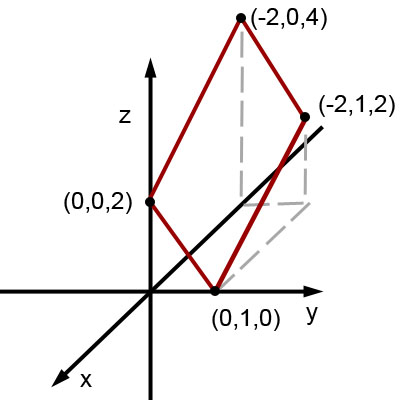
\includegraphics[width=0.35\textwidth]{WA06Solid.jpg}
  \end{center}
\end{figure}
\item We must integrate:
\begin{align*}
  \mathop{\int_{-2}^0 \! \int_0^1} (-x-2y+2 ) dydx 
  &= \int_{-2}^0 \big( -2xy -y^2 + 2y \big) \big|_0^1 dx \\
  &= \int_{-2}^0 \Big( -2x + 1  \Big) dx \\
  &= \Big(-x^2 + x \Big) \Big|_{-2}^0  \\  
  &= 0- \big(- (-2)^2 + (-2)\big)\\
  &= 0- \big(- 4 -2\big)\\
  &= 6
\end{align*}
\EEN
% ~~~~~~~~~~~~~~~~~~~~~~~~~~~~~~~~~~~~~~~~~~~~~~~~~~~~~~~~~~~~~~~~~~~~~~~~~~~~~~~~~
\item % TETRAHEDRON
\BEN
\item A sketch of the tetrahedron is below. 
\begin{figure}[h]
  \vspace{-1pt}
  \begin{center}
    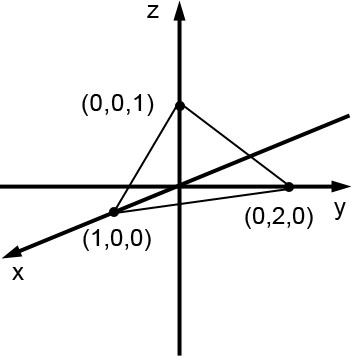
\includegraphics[width=0.35\textwidth]{WA06TetExample.jpg}
  \end{center}
\end{figure}
% ~  ~  ~  ~  ~  ~  ~  ~  ~  ~  ~  ~  ~  ~  ~  ~  ~  ~  ~  ~  ~  ~  ~  ~  
\item The tetrahedron has one side in the $xy$-plane. This side is bounded by the line that is the intersection between the $xy$-plane and the plane $z = 1 - x - y/2$. We can find this intersection by setting $z=0$,
\begin{align*}
  0 &= 1 - x - \frac{y}{2} \\
  x &= 1 - \frac{y}{2}.
\end{align*}
Therefore, the volume is the region under the plane $z = 1 - x - y/2$ and over  
\begin{align*}
  R = \{ (x,y) \ | \ 0 \le x \le 1- y/2, \ 0 \le y \le 2 \}.
\end{align*}
The double integral is 
\begin{align*}
  \mathop{\int_{0}^{2} \! \int_0^{1-y/2} } (1 - x - \frac{y}{2}) dxdy
\end{align*} 
% ~  ~  ~  ~  ~  ~  ~  ~  ~  ~  ~  ~  ~  ~  ~  ~  ~  ~  ~  ~  ~  ~  ~  ~  
\item The volume is the region under the plane $z = 1 - x - y/2$ and over  
\begin{align*}
  R = \{ (x,y) \ | \ 0 \le x \le 1, \ 0 \le y \le 2 - 2x \}.
\end{align*}
The double integral is 
\begin{align*}
  \mathop{\int_{0}^{1} \! \int_0^{2-2x} } (1 - x - \frac{y}{2}) dydx
\end{align*} 
\EEN
% ~~~~~~~~~~~~~~~~~~~~~~~~~~~~~~~~~~~~~~~~~~~~~~~~~~~~~~~~~~~~~~~~~~~~~~~~~~~~~~~~~
\item % DOUBLE INTEGRAL IS AREA IF F=1
Suppose that we subdivide region $R$ into a rectangular grid of sub-rectangles (as in Figure 3.2.5), so that we only consider the sub-rectangles that are completely enclosed in $R$. Then, the area of region $R$ is approximated by the double sum
\begin{align*}
  \sum_j\sum_i\Delta x_i \Delta y_j
\end{align*}
But if $f=1$ for all $x_i$ and $y_j$, this is equal to:
\begin{align}\label{abefaberabreabr}
  \sum_j\sum_i f(x_i,y_j) \Delta x_i \Delta y_j
\end{align}
where $x_i$ and $y_j$ is a point inside sub-rectangle $[x_i,x_{i+1}]\times[y_j,y_{j+1}]$. 
If we take smaller and smaller rectangles, so that the length of the longest diagonal of the sub-rectangles goes to zero, the sub-rectangles begin to fill more and more of the region $R$, and so the above sums approach the  \Emph{area} of region $R$. Since we have defined
\begin{align*}
  \mathop{\int \!\!\! \int} f(x,y) dA
\end{align*}
as the limit of Equation (\ref{abefaberabreabr}) as the longest diagonal goes to zero, and $f(x,y)=1$, the double integral 
\begin{align*}
  \mathop{\int \!\!\! \int} 1 dA
\end{align*}
is the area of region $R$. 
% ~~~~~~~~~~~~~~~~~~~~~~~~~~~~~~~~~~~~~~~~~~~~~~~~~~~~~~~~~~~~~~~~~~~~~~~~~~~~~~~~~
\item
\BEN
\item Substituting the expression for $u$ into the divergence equation yields
\begin{align*}
  0&= \nabla \cdot \MB{v} \\
  &= \px \big(u(x,y)\big) + \py \big(v(x,y)\big) \\
  &= \px (x^2 + y^2) + \frac{\partial v}{\partial y}\\
  &= 2x + \frac{\partial v}{\partial y} \\
   \frac{\partial v}{\partial y} &= -2x 
\end{align*}
Therefore, $v(x,y)$ is a function whose partial derivative with respect to $y$ is $-2x$. The \Emph{most general} form for $v(x,y)$ is obtained by integrating with respect to $y$:
\begin{align*}
 v(x,y) &= -2xy + f(x)
\end{align*}
where $f(x)$ is an unknown function of one variable, $x$. 
\item Using the same approach as we used for (a) yields
\begin{align*}
  0&= \nabla \cdot \MB{v} \\
  &= \px \big(u(x,y)\big) + \py \big(v(x,y)\big) \\
  &=  \frac{\partial u}{\partial x}+ 0\\
   \frac{\partial u}{\partial x} &= 0
\end{align*}
Therefore, $u(x,y)$ is a function whose partial derivative with respect to $x$ is $0$. The \Emph{most general} form for $u(x,y)$ is obtained by integrating with respect to $x$:
\begin{align*}
 u(x,y) &= g(y)
\end{align*}
where $g(y)$ is an unknown function of one variable, $y$. 
\EEN
% ~~~~~~~~~~~~~~~~~~~~~~~~~~~~~~~~~~~~~~~~~~~~~~~~~~~~~~~~~~~~~~~~~~~~~~~~~~~~~~~~~
\item % UPPER AND LOWER BOUNDS ARE FUNCTIONS
The curves $y=x^2$ and $x^2=y$ intersect at (0,0) and at (1,1). Integrating with respect to $y$ first yields
\begin{align*} 
  \mathop{\int_0^1 \!\!\! \int_{x^2}^{\sqrt{x}}} x^2+y^2 dydx 
  &= \int_0^1 \Big(yx^2 + \frac{y^3}{3} \Big)\Big|_{x^2}^{\sqrt{x}} dx \\
  &= \int_0^1 \Big(x^{5/2} + \frac{x^{3/2}}{3} - x^4 - \frac{x^6}{3}\Big) dx \\
  &= \Big( \frac{2}{7} x^{7/2} + \frac{2}{15}x^{5/2} - \frac{1}{5}x^5 - \frac{1}{21}x^7\Big)\Big|_0^1 \\
  &= \frac{2}{7} + \frac{2}{15} - \frac{1}{5} - \frac{1}{21} \\
  &= 6/35
\end{align*}
% ~~~~~~~~~~~~~~~~~~~~~~~~~~~~~~~~~~~~~~~~~~~~~~~~~~~~~~~~~~~~~~~~~~~~~~~~~~~~~~~~~
\item % CHANGING ORDER OF INTEGRATION
\BEN 
\item Integrating with respect to $y$ first yields
\begin{align*} 
  \mathop{\int_0^2 \!\!\! \int_0^{x^2}} x\sin (y) dydx 
  &= \int_0^2 -x\cos(y)\Big|_0^{x^2} dx \\
  &= - \int_0^2 \Big(x\cos(x^2)-1\Big) dx \\
  &= - \int_0^2x\cos(x^2) dx +  \int_0^2 1 \ dx \\    
  &= 2 - \int_0^2x\cos(x^2) dx 
\end{align*}
Now let $u=x^2$, so that $du = 2xdx$. Then 
\begin{align*} 
  2 - \int_0^2x\cos(x^2) dx  
  &=  2 - \int_0^4 x\cos(u)\Big(\frac{du}{2x}\Big)\\
  &=  2 - \frac{1}{2} \int_0^4 \cos(u)du \\
  &=  2 - \frac{1}{2} \sin(u) \Big|_0^4 \\
  &=  2 - \frac{1}{2} \sin(4) \\
  &\approx 2.3784
\end{align*}
\item Integrating with respect to $x$ first yields
\begin{align*} 
  \mathop{\int_0^4 \!\!\! \int_{\sqrt{y}}^{2} } x\sin (y) dxdy
  &= \int_0^4 \frac{x^2}{2}\sin(y)\Big|_{\sqrt{y}}^{2} \ dy \\
  &= \int_0^4 \frac{4-y}{2}\sin(y) dy \\
  &= 2 \int_0^4 \sin(y) dy - \frac{1}{2} \int_0^4 y\sin(y) dy \\
  &= 2 \big( - \cos(y) \big)\big|_0^4 - \frac{1}{2} \int_0^4 y\sin(y) dy \\
  &= 2 \big( - \cos(4) + 1 \big) - \frac{1}{2} \int_0^4 y\sin(y) dy \\
  &= 2  - 2\cos(4)  - \frac{1}{2} \int_0^4 y\sin(y) dy \\
\end{align*}
Now using integration by parts, with 
\begin{align*}
  u &= y, \quad dv = \sin(y)dy \\
  du &= dy, \quad v = -\cos(y)
\end{align*}
we obtain
\begin{align*} 
  \mathop{\int_0^4 \!\!\! \int_{\sqrt{y}}^{2} } x\sin (y) dxdy
  &= 2  - 2\cos(4)  - \frac{1}{2} \int_0^4 y\sin(y) dy \\
  &= 2  - 2\cos(4)  - \frac{1}{2}\Bigg( -y\cos(y)\Big|_0^4 - \int_0^4 \big(-\cos(y)\big) dy \Bigg) \\
  &= 2  - 2\cos(4)  - \frac{1}{2}\Bigg( -4\cos4 + \sin(y)\big|_0^4 \Bigg)  \\  
  &= 2  - 2\cos(4)  - \frac{1}{2}\Big( -4\cos4 + \sin(4)- 0 \Big)  \\  
  &= 2 - \frac{\sin(4)}{2}   \\  
  &\approx 2.3784
\end{align*}
\EEN
% ~~~~~~~~~~~~~~~~~~~~~~~~~~~~~~~~~~~~~~~~~~~~~~~~~~~~~~~~~~~~~~~~~~~~~~~~~~~~~~~~~
\item % CHANGING ORDER OF INTEGRATION, GENERAL F(X,Y)
The region over which we are integrating $f(x,y)$ is the shaded area below. 
\begin{figure}[h]
  \vspace{-1pt}
  \begin{center}
    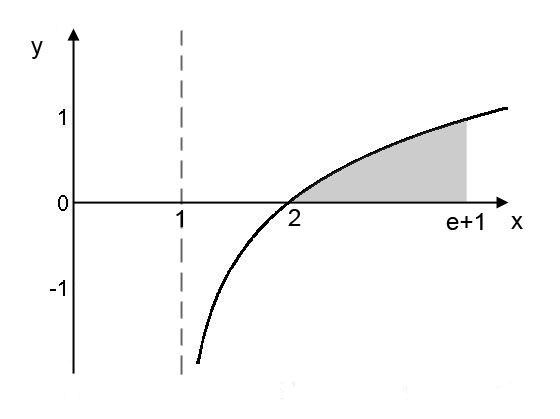
\includegraphics[width=0.55\textwidth]{Log.jpg}
  \end{center}
\end{figure}\\
The region is bounded by the lines $y=0$, $x=1+e$, and by the curve $y=\ln(x-1)$. Using horizontal slices, values of $y$ range from 0 to 1, and values of $x$ range from $e^y-1$ to $1+e$. The double integral becomes
\begin{align*}
  \mathop{\int_{0}^{1} \! \int_{e^y-1}^{1+e}} f(x,y) dydx .
\end{align*}
% ~~~~~~~~~~~~~~~~~~~~~~~~~~~~~~~~~~~~~~~~~~~~~~~~~~~~~~~~~~~~~~~~~~~~~~~~~~~~~~~~~
\item % BOUNDING AN INTEGRAL 
The integrand $f(x,y)$ has the property that 
\begin{align*}
  0 \le \sin(x+y) \le 1,
\end{align*}
because $x+y$ is between 0 and 2, and $\sin(2) < 1$. Then 
\begin{align*}
  0 = \iint\limits_D 0 dA  \le  \iint\limits_D f(x,y) dA \le  \iint\limits_D (1) dA = 1.
\end{align*}
% ~~~~~~~~~~~~~~~~~~~~~~~~~~~~~~~~~~~~~~~~~~~~~~~~~~~~~~~~~~~~~~~~~~~~~~~~~~~~~~~~~
\item % THE UNDEFINED INTEGRAL
%\BEN
%\item Integrating with respect to $y$ first yields
%\begin{align*} 
%  \iint\limits_R xe^{xy}dA
%  &=  \mathop{\int_0^1 \!\!\! \int_0^1} xe^{xy} dydx \\
%  &=  \int_0^1x \Bigg(\int_0^1e^{xy} dy \Bigg) dx \\
%  &=  \int_0^1 x \Bigg( \frac{1}{x}e^{xy} \Big|_{y=0}^{y=1}\Bigg) dx \\  
%  &=  \int_0^1 e^{xy} \Big|_0^1 dx \\  
%  &=  \int_0^1 (e^{x} - 1 )dx \\  
%  &=  (e^{x} - x) \Big|_0^1\\
%  &=  (e - 1) - (1 - 0) \\
%  &=  e  - 2  
%\end{align*}
Integrating with respect to $x$ first gives us the double integral
\begin{align*} 
  \iint\limits_D xe^{xy}dA &=  \mathop{\int_0^1 \!\!\! \int_0^1} xe^{xy} dxdy .
\end{align*}
Let's first consider the integration with respect to $x$ in isolation:
\begin{align*} 
  \int_0^1 xe^{xy} dx  .
  \end{align*}
Using integration by parts with $u=x$ and $dv = e^{xy}$, and treating $y$ as a constant, 
\begin{align*} 
  \int_0^1 xe^{xy} dx  
  &= x\Big(\frac{e^{xy}}{y}\Big)\Big|_0^1 - \int_0^1 \frac{1}{y}e^{xy}dx \\
  &= \frac{e^{y}}{y} -  \frac{1}{y} \int_0^1e^{xy}dx \\
  &= \frac{e^{y}}{y} -  \frac{1}{y^2} e^{xy}\big|_0^1\\
  &= \frac{e^{y}}{y} -  \frac{1}{y^2} (e^{y} - 1)
\end{align*}
We now must integrate 
\begin{align*} 
 \mathop{\int_0^1 \!\!\! \int_0^1} xe^{xy} dxdy &=\int_0^1 \Big(  \frac{e^{y}}{y} -  \frac{1}{y^2} (e^{y} - 1) \Big)dy\\
 &=\int_0^1   \frac{e^{y}}{y} dy - \int_0^1 \frac{e^{y} }{y^2}  dy + \int_0^1 \frac{1}{y^2}   dy
\end{align*}
The above three integrals do not exist! However, the double integral 
\begin{align*} 
  \mathop{\int_0^1 \!\!\! \int_0^1} xe^{xy} dxdy 
\end{align*}
exists, because the integrand is finite everywhere on $D$. The methods we are using in this course will not allow us to find the value of this double integral by first integrating with respect to $x$.

% ~~~~~~~~~~~~~~~~~~~~~~~~~~~~~~~~~~~~~~~~~~~~~~~~~~~~~~~~~~~~~~~~~~~~~~~~~~~~~~~~~
\EEN % END OF SOLUTIONS

\end{document}

